% ============================================================================
%   AAAI-style main paper draft for the GUDS-EDL architecture
%   Mathematical foundations, model architecture, and ISIC case study
%
%   File: guds_edl_report_en.tex
%   Version: 2.0 (Updated 06/2026)
%   Language: English
% ============================================================================

\documentclass[letterpaper]{article} % DO NOT CHANGE THIS
\usepackage{aaai}  % DO NOT CHANGE THIS
\usepackage{times}  % DO NOT CHANGE THIS
\usepackage{helvet}  % DO NOT CHANGE THIS
\usepackage{courier}  % DO NOT CHANGE THIS
\usepackage[hyphens]{url}  % DO NOT CHANGE THIS
\usepackage{graphicx} % DO NOT CHANGE THIS
\urlstyle{rm} % DO NOT CHANGE THIS
\def\UrlFont{\rm}  % DO NOT CHANGE THIS
\frenchspacing  % DO NOT CHANGE THIS
\setlength{\pdfpagewidth}{8.5in} % DO NOT CHANGE THIS
\setlength{\pdfpageheight}{11in}
\setcounter{secnumdepth}{2}
%%%%%%%%%%
% PDFINFO for PDFLATEX
\pdfinfo{
/Title (GUDS-EDL: Generalized Uncertainty-Guided Dynamic Sparsification for Evidential Long-Tailed Learning)
/Author (Anonymous Authors)
}
%%%%%%%%%%
 % DO NOT CHANGE THIS

% --- Additional Packages ---
\usepackage[utf8]{inputenc}
\usepackage[english]{babel}
\usepackage{amsmath, amssymb, amsthm, bm}
\usepackage{booktabs}
\usepackage{multirow}
\usepackage{array}
\usepackage{adjustbox}
\usepackage{placeins}
\usepackage{stfloats}
\usepackage{algorithm}
\usepackage{algorithmic}
\usepackage{enumitem}
\usepackage{tikz}
\usetikzlibrary{arrows.meta, positioning, calc}
\usepackage[table]{xcolor}
\usepackage{colortbl}
\usepackage[colorlinks=true,linkcolor=black,citecolor=blue,urlcolor=blue]{hyperref}

\newcolumntype{C}{>{\centering\arraybackslash}c}

% --- Custom commands ---
\newcommand{\Dir}{\text{Dir}}
\newcommand{\KL}{\text{KL}}
\newcommand{\R}{\mathbb{R}}
\newcommand{\E}{\mathbb{E}}
\newcommand{\Norm}{\text{Norm}}
\newcommand{\softplus}{\text{Softplus}}
\DeclareMathOperator*{\argmax}{arg\,max}

\hbadness=10000
\vbadness=10000
\hfuzz=10pt
\vfuzz=4pt
\raggedbottom
\setlength{\textfloatsep}{10pt plus 2pt minus 3pt}
\setlength{\dbltextfloatsep}{10pt plus 2pt minus 3pt}
\setlength{\floatsep}{8pt plus 2pt minus 2pt}
\setlength{\dblfloatsep}{8pt plus 2pt minus 2pt}

% ============================================================================
\title{GUDS-EDL: Generalized Uncertainty-Guided Dynamic Sparsification for Evidential Long-Tailed Learning}
\author{Anonymous Authors}

\begin{document}
\maketitle

\begin{abstract}
Extreme imbalanced classification requires rare-event sensitivity, uncertainty awareness, and hardware-compatible structured sparsity. We propose \textbf{GUDS-EDL}, an uncertainty-guided sparse evidential framework that couples Dirichlet-derived structural signals with valid-block 2:4 sparsity. GUDS-EDL updates latent topology scores with two first-order modules: a signed evidential-risk pruner for active connections and an evidence-seeking regrower for candidate connections. Mask refresh uses vacuity, expected entropy, and KL-based evidence-growth saliency, while a capped imbalance-aware evidential objective supports rare-event learning without changing the Dirichlet prior. We instantiate GUDS-EDL on ISIC 2024 as an extreme-prevalence medical screening case study. Claims are limited to this setting; ablations, broader long-tailed and anomaly-detection benchmarks, and hardware-kernel validation are treated as protocols unless explicitly reported.
\end{abstract}

\section{Introduction}
Extreme imbalanced classification appears in rare-event screening, industrial inspection, fraud detection, and other settings where minority errors are costly. In these regimes, a model must classify rare cases, express uncertainty under weak evidence, and remain compatible with deployment-constrained inference. Standard softmax classifiers can become overconfident under class imbalance and dataset shift~\cite{guo2017calibration}, while dense models may be inefficient when structured sparsity is required.

Evidential Deep Learning (EDL) provides Dirichlet-derived quantities such as vacuity and expected categorical entropy~\cite{sensoy2018evidential,malinin2018predictive}, but these signals are typically used only for prediction, calibration, or rejection. Dynamic Sparse Training (DST) adapts sparse topology during optimization~\cite{evci2020rigging}, but most topology rules rely on magnitude or task-gradient criteria and do not explicitly use evidential uncertainty. This leaves a gap: uncertainty-aware classifiers rarely adapt their sparse structure, while sparse learners remain uncertainty-agnostic.

We introduce \textbf{GUDS-EDL}, a valid-block 2:4 dynamic sparse evidential framework. The method updates latent topology scores through a signed evidential-risk pruner and an evidence-seeking regrower, then refreshes the mask by Top-2 selection within each eligible 4-block. Our contributions are: (i) a capped imbalance-aware evidential objective, (ii) a rank-normalized first-order topology update driven by Dirichlet-derived signals, and (iii) a conservative ISIC 2024 case study that separates reported evidence from broader validation protocols.

\section{Related Work}
\paragraph{Long-Tailed and Imbalanced Learning.} Long-tailed recognition is commonly addressed by re-weighting, margin adjustment, logit correction, classifier decoupling, and contrastive learning~\cite{cui2019class,cao2019learning,menon2021long,ren2020balanced,kang2019decoupling,cui2021parametric}. Architectures such as BBN further improve head-tail trade-offs~\cite{zhou2020bbn}. GUDS-EDL instead uses evidential structural signals to adapt sparse topology under imbalance.

\paragraph{Evidential and Dirichlet Uncertainty.} Evidential Deep Learning~\cite{sensoy2018evidential} and related Prior/Posterior Networks~\cite{malinin2018predictive} formulate classification via a Dirichlet distribution, enabling single-pass uncertainty estimation. Recent variants such as Fisher EDL~\cite{deng2023fisher}, R-EDL~\cite{chen2023redl}, Flexible EDL~\cite{yoon2025flexible}, ANEDL~\cite{yu2024anedl}, and Evidence Contraction~\cite{wu2024evidence} improve or analyze evidence learning. Recent critiques caution against over-interpreting EDL as true Bayesian uncertainty~\cite{shen2024mirage}. GUDS-EDL follows this caution and uses Dirichlet vacuity and expected entropy as structural proxies, not Bayesian guarantees.

\paragraph{Calibration and Selective Prediction.} Reliable model use requires calibrated confidence~\cite{guo2017calibration} and the ability to abstain on ambiguous samples, formalized by selective classification and metrics like AURC~\cite{geifman2017selective,geifman2019selectivenet,ding2020revisiting,traub2024overcoming}. We therefore report uncertainty metrics together with operating-point metrics rather than relying on overall accuracy.

\paragraph{Dynamic Sparse Training and Structured Sparsity.} Dynamic sparse training maintains sparse connectivity throughout optimization~\cite{dettmers2019sparse,evci2020rigging,li2025pffdst}. Hardware-compatible sparsity constraints, including NVIDIA's 2:4 pattern, motivate structured sparse training and inference when appropriate kernels are used~\cite{mishra2021accelerating,lasby2023srigl}. Existing long-tailed methods rebalance objectives, evidential methods estimate uncertainty without changing topology, and DST methods evolve masks without uncertainty awareness. GUDS-EDL fills this gap by using evidential uncertainty itself as the signal for structured sparse topology adaptation under extreme imbalance.

\section{Method}

\subsection{Evidential Prediction and Uncertainty Proxies}
For logits $\bm{z}\in\mathbb{R}^K$, GUDS-EDL maps each class logit to non-negative evidence using Softplus,
\begin{equation}
e_c=\log(1+\exp z_c),\quad \alpha_c=e_c+1,\quad S=\sum_{c=1}^K\alpha_c .
\end{equation}
The predictive mean is $\hat p_c=\alpha_c/S$. With uniform base rate $a_c=1/K$, the subjective-logic form matches the Dirichlet mean: $\hat p_c=b_c+a_cu_e=(e_c+1)/S$, where $b_c=e_c/S$ and $u_e=K/S$. Following recent critiques on Bayesian epistemic bounds~\cite{shen2024mirage}, we use $u_e$ as a low-evidence structural proxy and use expected categorical entropy
\begin{equation}
u_a=\sum_{c=1}^K\frac{\alpha_c}{S}\left[\psi(S+1)-\psi(\alpha_c+1)\right]
\end{equation}
as an ambiguity proxy. These are Dirichlet-derived structural signals, not exact Bayesian posterior uncertainty.

\begin{figure}[t]
\centering
\resizebox{\columnwidth}{!}{%
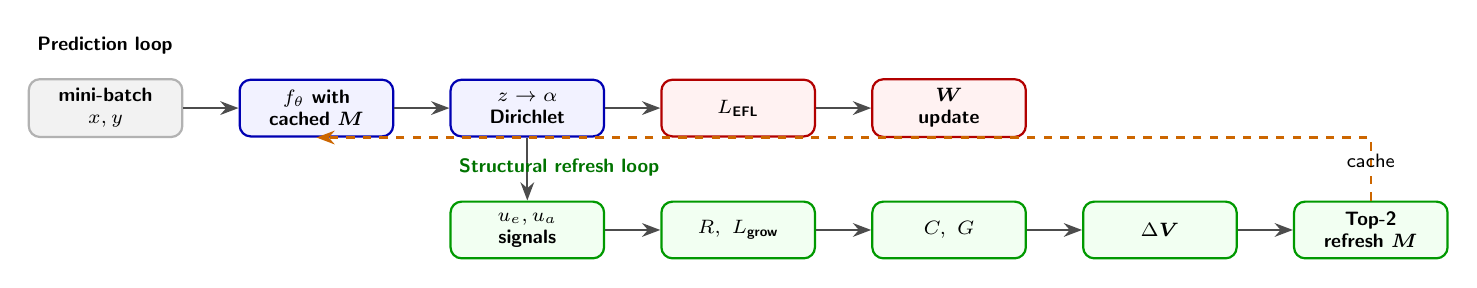
\begin{tikzpicture}[
    node distance=0.8cm and 0.7cm,
    box/.style={
        draw=blue!70!black,
        fill=blue!5,
        rounded corners,
        align=center,
        minimum width=1.95cm,
        minimum height=0.72cm,
        font=\scriptsize\sffamily\bfseries,
        thick
    },
    opt/.style={
        draw=red!70!black,
        fill=red!5,
        rounded corners,
        align=center,
        minimum width=1.95cm,
        minimum height=0.72cm,
        font=\scriptsize\sffamily\bfseries,
        thick
    },
    struct/.style={
        draw=green!60!black,
        fill=green!5,
        rounded corners,
        align=center,
        minimum width=1.95cm,
        minimum height=0.72cm,
        font=\scriptsize\sffamily\bfseries,
        thick
    },
    arrow/.style={
        ->,
        >=Stealth,
        thick,
        draw=black!70
    },
    feedback/.style={
        ->,
        >=Stealth,
        thick,
        dashed,
        draw=orange!80!black
    }
]

% Nodes
\node (x) [box, fill=gray!10, draw=gray!60] {mini-batch\\$x,y$};
\node (f) [box, right=of x] {$f_\theta$ with\\cached $\bm{M}$};
\node (za) [box, right=of f] {$z\to\alpha$\\Dirichlet};
\node (loss) [opt, right=of za] {$L_{\text{EFL}}$};
\node (wup) [opt, right=of loss] {$\bm{W}$\\update};

\node (sig) [struct, below=of za] {$u_e,u_a$\\signals};
\node (risk) [struct, right=of sig] {$R,\ L_{\text{grow}}$};
\node (cg) [struct, right=of risk] {$C,\ G$};
\node (dv) [struct, right=of cg] {$\Delta\bm{V}$};
\node (top) [struct, right=of dv] {Top-2\\refresh $\bm{M}$};

% Paths
\draw [arrow] (x) -- (f);
\draw [arrow] (f) -- (za);
\draw [arrow] (za) -- (loss);
\draw [arrow] (loss) -- (wup);
\draw [arrow] (za) -- (sig);
\draw [arrow] (sig) -- (risk);
\draw [arrow] (risk) -- (cg);
\draw [arrow] (cg) -- (dv);
\draw [arrow] (dv) -- (top);
\draw [feedback] (top.north) |- node[above, pos=0.18, font=\scriptsize\sffamily] {cache} (f.south);
\node[font=\scriptsize\sffamily\bfseries, anchor=south west] at ($(x.north west)+(0,0.18)$) {Prediction loop};
\node[font=\scriptsize\sffamily\bfseries, anchor=south west, green!45!black] at ($(sig.north west)+(0,0.18)$) {Structural refresh loop};

\end{tikzpicture}%
}
\caption{Two-loop GUDS-EDL mechanism. The prediction loop updates active weights under a cached mask; the structural refresh loop uses Dirichlet-derived signals to update latent topology scores and refresh the valid-block 2:4 mask.}
\label{fig:overview}
\end{figure}


\subsection{2:4 Dynamic Sparse Topology}
We use a hardware-compatible 2:4 pattern on eligible complete blocks. Each wrapped layer has active weights $\bm{W}$ and latent topology scores $\bm{V}$:
\begin{equation}
\bm{W}^{(\ell)}_{\mathrm{eff}}=\bm{W}^{(\ell)}\odot\bm{M}^{(\ell)},\quad
\bm{M}^{(\ell)}_B=\operatorname{Top2}(\bm{V}^{(\ell)}_B),\ |B|=4 .
\end{equation}
Trailing coordinates outside complete 4-blocks are excluded from 2:4 accounting and kept dense; auxiliary padding is non-trainable and cannot consume active slots. Masks are refreshed at structural update points using an amortized proxy batch.

\subsection{Signed Uncertainty-Guided Pruning}
On a proxy batch $\mathcal{B}$, define the evidential risk ratio
\begin{equation}
R_{\mathcal{B}}=\frac{1}{|\mathcal{B}|}\sum_{n\in\mathcal{B}}\frac{u_a^{(n)}}{u_e^{(n)}+\epsilon}.
\end{equation}
With the current mask fixed, removing an active connection gives $\Delta R_{\mathcal B}\approx -w_{ij}\partial R_{\mathcal B}/\partial w_{\mathrm{eff},ij}$. Thus positive $w_{ij}\partial R_{\mathcal B}/\partial w_{\mathrm{eff},ij}$ means removal locally decreases batch evidential risk to first order. The pruning score is
\begin{equation}
C_{ij}=\operatorname{Rank}_{\ell}\left([w_{ij}\partial R_{\mathcal B}/\partial w_{\mathrm{eff},ij}]_+\right),
\end{equation}
where $[x]_+=\max(x,0)$ is a positive-part gate, not a neural ReLU activation.

\subsection{Class-Conditioned Evidence-Seeking Regrowth}
For regrowth, we use a scalar sample gate on the KL divergence to the uniform Dirichlet prior:
\begin{equation}
L_{\mathrm{grow}}=\frac{1}{|\mathcal{B}|}\sum_{n\in\mathcal{B}} g_n^{\mathrm{grow}}
\KL(\Dir(\bm{\alpha}^{(n)})\parallel\Dir(\mathbf{1})),\quad
g_n^{\mathrm{grow}}=\tilde{\omega}_{y_n}u_e^{(n)} .
\end{equation}
Class conditioning changes only the scalar gate, not $\bm{\alpha}$. The regrowth score is
\begin{equation}
G_{ij}=\operatorname{Rank}_{\ell}\left(\left|\partial L_{\mathrm{grow}}/\partial w_{\mathrm{eff},ij}\right|\right).
\end{equation}
Ordinary gradients with respect to inactive weights are zero under masking, but structural refresh retains dense proxy gradients with respect to $\bm{W}_{\mathrm{eff}}$; dormant candidates therefore receive structural saliency estimates.

The latent topology update combines active-link competition and dormant-link exploration:
\begin{equation}
    \Delta\bm{V}=\bm{M}\odot(\bm{G}-\bm{C})+(1-\bm{M})\odot(\rho\bm{G}+\bm{\xi}),
\end{equation}
followed by momentum, score clipping, and Top-2 mask refresh. Thus pruning pressure affects only active links, while dormant links are driven by regrowth and small tie-breaking exploration. Rank normalization aligns layer-wise saliency scales; it is not an optimality guarantee.

\subsection{Imbalance-Aware Evidential Objective}
We use an imbalance-aware evidential objective with square-root frequency dampening:
\begin{equation}
L_{\mathrm{EFL}}=\frac{1}{N}\sum_{n=1}^N\mathcal{F}_n(t)
\left[
\tilde{\omega}_{y_n}L_{\mathrm{CE}}^{(n)}
+\lambda_{\mathrm{KL}}\mu(t)\Lambda_{\mathrm{asym}}^{(n)}L_{\mathrm{KL}}^{(n)}
\right],
\end{equation}
where $\tilde{\omega}_{c}=\min(\sqrt{N_{\mathrm{major}}/N_c},\omega_{\max})$, $\mathcal{F}_n(t)=(1-\mathrm{sg}[\hat p_{y_n}])^{\gamma(t)}$, and $\Lambda_{\mathrm{asym}}^{(n)}=\min(\tilde{\omega}_{y_n},\Lambda_{\max})$. The CE and KL multipliers are separated to avoid double-counting class-frequency pressure. The stop-gradient focal term changes sample emphasis without adding a confidence-derivative path. Full KL and warmup details are left to the Supplementary Material.

\subsection{Bias-Corrected Calibration and Training Loop}
Post-hoc calibration is applied to logits before the Softplus evidence map. Because this changes both predictive probabilities and Dirichlet strength, we treat it as evidential post-hoc calibration rather than ordinary softmax temperature scaling. Thresholds are selected on validation probabilities and do not recalibrate the underlying evidence values.

Training proceeds in three distinct stages: dense warmup, epoch-level topology adaptation, and masked evidential optimization. After warmup, a proxy batch is used once per epoch to compute pruning and regrowth scores, update latent vitality scores, and refresh 2:4 masks. Standard mini-batch training then updates only active weights under the fixed mask for the remainder of the epoch.

\section{Experimental Setup: Initial ISIC 2024 Case Study}
We instantiate our method on the ISIC 2024 Challenge dataset (3D-TBP images with 0.15\% minority prevalence). We use a stratified 70/5/5/20 train/validation/calibration/test split grouped by patient. The validation partition selects operating thresholds, the calibration partition fits post-hoc calibration when used, and the test partition is a local hold-out set. We compare against Fisher EDL~\cite{deng2023fisher}, Flexible EDL~\cite{yoon2025flexible}, and R-EDL~\cite{chen2023redl}. Models are evaluated using Sensitivity, Specificity, F2, Macro-AUROC, pAUC$_{0.80}$, PR-AUC, ECE, Minority ECE, and AURC.

\section{Results}
Under 0.15\% prevalence, overall accuracy is uninformative. We therefore report operating-point Sensitivity/Specificity, high-recall Specificity, pAUC over the high-TPR region, PR-AUC, ECE, Minority ECE, and AURC. AURC is interpreted together with working-point metrics because majority-dominated test sets can mask minority-class behavior.

\begin{table*}[!t]
\centering
\caption{ISIC 2024 Case Study: Classification performance comparison under Adaptive Operating Modes. The extreme class imbalance (0.15\% rare-event prevalence) renders standard default thresholds ($\tau=0.50$) unviable. The Balanced Utility mode maximizes the arithmetic mean of Sensitivity and Specificity, while the High-Recall Fail-Safe mode targets a minimum diagnostic Sensitivity of 80\% to minimize false negatives.}
\label{tab:results_classification}
\renewcommand{\arraystretch}{1.12}
\setlength{\tabcolsep}{3.2pt}
\begin{adjustbox}{max width=\textwidth}
\begin{tabular}{l C C C C C C C C C}
\toprule
 & \multicolumn{3}{c}{\textbf{Default Threshold ($\tau = 0.50$)}} & \multicolumn{3}{c}{\textbf{Balanced Utility}} & \multicolumn{3}{c}{\textbf{High-Recall Fail-Safe}} \\
\cmidrule(lr){2-4} \cmidrule(lr){5-7} \cmidrule(lr){8-10}
\textbf{Model} & \textbf{Sens.} $\uparrow$ & \textbf{Spec.} $\uparrow$ & \textbf{F2} $\uparrow$ & \textbf{Sens.} $\uparrow$ & \textbf{Spec.} $\uparrow$ & \textbf{F2} $\uparrow$ & \textbf{Sens.} $\uparrow$ & \textbf{Spec.} $\uparrow$ & \textbf{F2} $\uparrow$ \\
\midrule
Fisher EDL   & $0.3117$ & $0.9864$ & $0.0978$ & $0.7273$ & $0.8739$ & $0.0323$ & $0.8052$ & $0.7393$ & $0.0177$ \\
Flexible EDL & $0.3117$ & $0.9892$ & $0.1147$ & $0.8182$ & $0.8203$ & $0.0258$ & $0.8182$ & $0.8203$ & $0.0258$ \\
R-EDL        & $0.3506$ & $0.9796$ & $0.0805$ & $0.7662$ & $0.8357$ & $0.0264$ & $0.8052$ & $0.7473$ & $0.0182$ \\
\midrule
\textbf{GUDS-EDL (Ours)} & $\mathbf{0.4286}$ & $0.9854$ & $\mathbf{0.1265}$ & $\mathbf{0.8312}$ & $\mathbf{0.8828}$ & $\mathbf{0.0396}$ & $0.8052$ & $\mathbf{0.9030}$ & $\mathbf{0.0459}$ \\
\bottomrule
\end{tabular}
\end{adjustbox}

\vspace{0.75em}
\caption{Threshold-independent calibration, ranking, and uncertainty metrics. Lower ECE, Minority ECE, and AURC represent better confidence calibration and superior selective classification (abstention) capacity.}
\label{tab:results_uncertainty}
\renewcommand{\arraystretch}{1.12}
\setlength{\tabcolsep}{3.0pt}
\begin{adjustbox}{max width=\textwidth}
\begin{tabular}{l C C C C C C C C}
\toprule
\textbf{Model} & \textbf{Macro-AUROC} $\uparrow$ & \textbf{pAUC$_{0.80}$} $\uparrow$ & \textbf{PR-AUC} $\uparrow$ & \textbf{ECE} $\downarrow$ & \textbf{Minority ECE} $\downarrow$ & \textbf{AURC} $\downarrow$ & \textbf{Mean $u_e$} & \textbf{Mean $u_a$} \\
\midrule
Fisher EDL   & $0.8660$ & $0.1048$ & $0.0266$ & $0.2139$ & $\mathbf{0.3491}$ & $0.0009$ & $0.3822$ & $0.4453$ \\
Flexible EDL & $0.8835$ & $0.1138$ & $0.0251$ & $0.1097$ & $0.6101$ & $\mathbf{0.0003}$ & $0.2068$ & $0.2913$ \\
R-EDL        & $0.8741$ & $0.1126$ & $0.0183$ & $\mathbf{0.0989}$ & $0.3583$ & $0.0018$ & $0.2285$ & $\mathbf{0.1298}$ \\
\midrule
\textbf{GUDS-EDL (Ours)} & $\mathbf{0.9088}$ & $\mathbf{0.1296}$ & $\mathbf{0.0297}$ & $0.1113$ & $0.5089$ & $\mathbf{0.0003}$ & $0.2112$ & $0.2985$ \\
\bottomrule
\end{tabular}
\end{adjustbox}
\end{table*}


GUDS-EDL demonstrates strong ranking and high-recall operating performance. As detailed in Table~\ref{tab:results_classification}, under the High-Recall Fail-Safe mode (Sensitivity at least 80\%), GUDS-EDL maintains a Sensitivity of 0.8052 while achieving a Specificity of 0.9030. This exceeds Fisher EDL (0.7393), R-EDL (0.7473), and Flexible EDL (0.8203) at the same operating regime. The result is consistent with the design goal of improving rare-event decision behavior under structured sparsity, although component-level attribution requires the ablation protocol described outside the main results.

Furthermore, threshold-independent metrics in Table~\ref{tab:results_uncertainty} reinforce this advantage. GUDS-EDL achieves the highest Macro-AUROC (0.9088), pAUC$_{0.80}$ (0.1296), and PR-AUC (0.0297). However, calibration remains a caveat: GUDS-EDL does not dominate global ECE or Minority ECE. Thus, the primary empirical claim is improved rare-event ranking and high-recall operating specificity, not universal calibration superiority.

Finally, the 20\% test set contains only 77 positive cases. The 95\% Wilson interval for 0.8052 Sensitivity is [0.703, 0.878], so a few false negatives can shift the metric. At Sensitivity 0.8052, Specificity 0.9030, and prevalence 0.15\%, PPV is approximately 1.23\%; the plausible use case is triage-level filtering, with clinical deployment requiring decision-curve and net-benefit analysis.

\section{Limitations and Conclusion}
GUDS-EDL is currently validated mainly on ISIC 2024. The method enforces a fixed Top-2-of-4 pattern after warmup, while annealed sparsity schedules may be beneficial. Valid-block 2:4 sparsity reduces active density in wrapped layers, but real acceleration requires compatible sparse Tensor Core kernels. Minority-class calibration also remains challenging under extreme prevalence shifts.

We introduced GUDS-EDL as a conservative uncertainty-guided dynamic sparse evidential framework. The method uses Dirichlet vacuity and expected entropy to guide valid-block 2:4 topology adaptation, improving rare-event ranking and high-recall operating specificity in the reported case study. Broader long-tailed, anomaly-detection, multi-seed, ablation, and hardware-kernel validation remain necessary before domain-general claims.

\begin{thebibliography}{10}\itemsep=-1pt

\bibitem[\protect\citeauthoryear{Guo et al.}{2017}]{guo2017calibration}
C.~Guo, G.~Pleiss, Y.~Sun, and K.~Q.~Weinberger.
\newblock On calibration of modern neural networks.
\newblock In {\em ICML}, 2017.

\bibitem[\protect\citeauthoryear{Sensoy, Kaplan, and Kandemir}{2018}]{sensoy2018evidential}
M.~Sensoy, L.~Kaplan, and M.~Kandemir.
\newblock Evidential deep learning to quantify classification uncertainty.
\newblock In {\em NeurIPS}, 2018.

\bibitem[\protect\citeauthoryear{Malinin and Gales}{2018}]{malinin2018predictive}
A.~Malinin and M.~Gales.
\newblock Predictive uncertainty estimation via prior networks.
\newblock In {\em NeurIPS}, 2018.

\bibitem[\protect\citeauthoryear{Evci et al.}{2020}]{evci2020rigging}
U.~Evci, T.~Gale, J.~Amdrup, M.~Riabkov, and E.~Righart.
\newblock Rigging the lottery: Making all tickets winners.
\newblock In {\em ICML}, 2020.

\bibitem[\protect\citeauthoryear{Cui et al.}{2019}]{cui2019class}
Y.~Cui, M.~Jia, T.-Y.~Lin, Y.~Song, and S.~Belongie.
\newblock Class-balanced loss based on effective number of samples.
\newblock In {\em CVPR}, 2019.

\bibitem[\protect\citeauthoryear{Cao et al.}{2019}]{cao2019learning}
K.~Cao, C.~Wei, A.~Gaidon, N.~Arechiga, and T.~Ma.
\newblock Learning imbalanced datasets with label-distribution-aware margin loss.
\newblock In {\em NeurIPS}, 2019.

\bibitem[\protect\citeauthoryear{Menon et al.}{2021}]{menon2021long}
A.~K. Menon, S.~Jayasumana, A.~S. Rawat, H.~Jain, A.~Veit, and S.~Kumar.
\newblock Long-tail learning via logit adjustment.
\newblock In {\em ICLR}, 2021.

\bibitem[\protect\citeauthoryear{Ren et al.}{2020}]{ren2020balanced}
J.~Ren, C.~Yu, S.~Sheng, X.~Ma, H.~Zhao, S.~Yi, and H.~Li.
\newblock Balanced meta-softmax for long-tailed visual recognition.
\newblock In {\em NeurIPS}, 2020.

\bibitem[\protect\citeauthoryear{Kang et al.}{2020}]{kang2019decoupling}
B.~Kang, S.~Xie, M.~Rohrbach, Z.~Yan, A.~Gordo, J.~Feng, and Y.~Kalantidis.
\newblock Decoupling representation and classifier for long-tailed recognition.
\newblock In {\em ICLR}, 2020.

\bibitem[\protect\citeauthoryear{Zhou et al.}{2020}]{zhou2020bbn}
B.~Zhou, Q.~Cui, X.-S.~Wei, and Z.-M.~Chen.
\newblock BBN: Bilateral-branch network with cumulative learning for long-tailed visual recognition.
\newblock In {\em CVPR}, 2020.

\bibitem[\protect\citeauthoryear{Cui et al.}{2021}]{cui2021parametric}
J.~Cui, Z.~Zhong, S.~Liu, B.~Yu, and J.~Jia.
\newblock Parametric contrastive learning.
\newblock In {\em ICCV}, 2021.

\bibitem[\protect\citeauthoryear{Deng et al.}{2023}]{deng2023fisher}
D.~Deng, G.~Chen, Y.~Yu, F.~Liu, and P.-A. Heng.
\newblock Uncertainty estimation by Fisher information-based evidential deep learning.
\newblock In {\em ICML}, PMLR, 2023.

\bibitem[\protect\citeauthoryear{Chen, Gao, and Xu}{2024}]{chen2023redl}
M.~Chen, J.~Gao, and C.~Xu.
\newblock R-EDL: Relaxing nonessential settings of evidential deep learning.
\newblock In {\em ICLR}, 2024.

\bibitem[\protect\citeauthoryear{Yoon and Kim}{2025}]{yoon2025flexible}
T.~Yoon and H.~Kim.
\newblock Uncertainty estimation by flexible evidential deep learning.
\newblock {\em arXiv preprint arXiv:2510.18322}, 2025.

\bibitem[\protect\citeauthoryear{Yu et al.}{2024}]{yu2024anedl}
Y.~Yu, D.~Deng, F.~Liu, Y.~Jin, Q.~Dou, G.~Chen, and P.-A. Heng.
\newblock ANEDL: Adaptive negative evidential deep learning for open-set semi-supervised learning.
\newblock In {\em AAAI}, 2024.

\bibitem[\protect\citeauthoryear{Wu et al.}{2024}]{wu2024evidence}
Y.~Wu, B.~Shi, B.~Dong, Q.~Zheng, and H.~Wei.
\newblock The evidence contraction issue in deep evidential regression: Discussion and solution.
\newblock In {\em AAAI}, 2024.

\bibitem[\protect\citeauthoryear{Shen et al.}{2024}]{shen2024mirage}
M.~Shen, J.~J. Ryu, S.~Ghosh, Y.~Bu, P.~Sattigeri, S.~Das, and G.~W. Wornell.
\newblock Are uncertainty quantification capabilities of evidential deep learning a mirage?
\newblock In {\em NeurIPS}, 2024.

\bibitem[\protect\citeauthoryear{Geifman and El-Yaniv}{2017}]{geifman2017selective}
Y.~Geifman and R.~El-Yaniv.
\newblock Selective classification for deep neural networks.
\newblock In {\em NeurIPS}, 2017.

\bibitem[\protect\citeauthoryear{Geifman and El-Yaniv}{2019}]{geifman2019selectivenet}
Y.~Geifman and R.~El-Yaniv.
\newblock SelectiveNet: A deep neural network with an integrated reject option.
\newblock In {\em ICML}, 2019.

\bibitem[\protect\citeauthoryear{Ding et al.}{2020}]{ding2020revisiting}
Y.~Ding, J.~Liu, J.~Xiong, and Y.~Shi.
\newblock Revisiting the evaluation of uncertainty estimation and its application to explore model complexity-uncertainty trade-off.
\newblock In {\em CVPR Workshops}, 2020.

\bibitem[\protect\citeauthoryear{Traub et al.}{2024}]{traub2024overcoming}
J.~Traub, T.~J. Bungert, C.~T. L{\"u}th, M.~Baumgartner, K.~H. Maier-Hein, L.~Maier-Hein, and P.~F. Jaeger.
\newblock Overcoming common flaws in the evaluation of selective classification systems.
\newblock In {\em NeurIPS}, 2024.

\bibitem[\protect\citeauthoryear{Dettmers and Zettlemoyer}{2019}]{dettmers2019sparse}
T.~Dettmers and L.~Zettlemoyer.
\newblock Sparse networks from scratch: Faster training without losing performance.
\newblock In {\em ICLR Workshop}, 2019.

\bibitem[\protect\citeauthoryear{Li et al.}{2025}]{li2025pffdst}
L.~Li, H.~Yang, J.~Guo, H.~Yu, M.~Qin, and T.~Zhang.
\newblock An efficient and accurate dynamic sparse training framework based on parameter-freezing.
\newblock In {\em AAAI}, 2025.

\bibitem[\protect\citeauthoryear{Lasby et al.}{2024}]{lasby2023srigl}
M.~Lasby, A.~Golubeva, U.~Evci, M.~Nica, and Y.~Ioannou.
\newblock Dynamic sparse training with structured sparsity.
\newblock In {\em ICLR}, 2024.

\bibitem[\protect\citeauthoryear{Mishra et al.}{2021}]{mishra2021accelerating}
Asit Mishra, Jorge Albericio Latorre, Jeff Pool, Darko Stosic, Dusan Stosic, Ganesh Venkatesh, Chong Yu, and Paulius Micikevicius.
\newblock Accelerating sparse deep neural networks.
\newblock {\em arXiv preprint arXiv:2104.08378}, 2021.

\end{thebibliography}
\end{document}
